% ===================================================================
% Manuscript: GHZ-Based Quantum Secret Sharing
% Target: AVS Quantum Science (AIP Publishing, Q1)
% Format: Single column (preprint)
% ===================================================================
\documentclass[aip, amsmath, amssymb, preprint, longbibliography]{revtex4-2}

% --- Packages ---
\usepackage{graphicx}
\usepackage{dcolumn}
\usepackage{bm}
\usepackage{hyperref}
\usepackage{xcolor}
\usepackage{booktabs}
\usepackage{multirow}
\usepackage{siunitx}
\usepackage{braket}
\usepackage{float}

% --- Custom commands ---
\newcommand{\ghz}{\text{GHZ}}
\newcommand{\cnot}{\textsc{cnot}}
\newcommand{\qber}{\text{QBER}}
\newcommand{\fid}{\mathcal{F}}

% ===================================================================
\begin{document}

\title{Comprehensive Noise-Aware Simulation and Hardware Validation of
GHZ-Based Quantum Secret Sharing on Superconducting Processors}

\author{Tanvir Hassan}
\email{tanvir6307@gmail.com}
\affiliation{Department of Physics, Jagannath University, Dhaka 1100, Bangladesh}


% ===================================================================
% ABSTRACT
% ===================================================================
\begin{abstract}
Quantum secret sharing (QSS) extends classical secret splitting to the
quantum domain by exploiting multipartite entanglement, yet its practical
viability on noisy intermediate-scale quantum (NISQ) hardware remains
insufficiently characterized. We present a comprehensive density-matrix
simulation of the Hillery--Bu\v{z}ek--Berthiaume (HBB) protocol using
Greenberger--Horne--Zeilinger (GHZ) states as the entanglement resource,
incorporating eight physically motivated noise channels:
thermal relaxation ($T_1/T_2$), depolarizing gate errors, coherent
over-rotation, $ZZ$ crosstalk, leakage to non-computational levels,
$1/f^\alpha$ dephasing, collective correlated dephasing, and
state-preparation-and-measurement (SPAM) errors. All noise parameters are
anchored to independently calibrated data from IBM Quantum Falcon-class
processors. For three-party sharing we obtain a GHZ state fidelity of
$\mathcal{F}=0.950\pm0.002$ and a protocol success rate of
$89.7\%\pm0.2\%$, with fidelity scaling well described by an exponential
decay $\mathcal{F}(n)=0.357\,e^{-0.330\,n}+0.819$ ($R^2=0.997$) up to
$n=7$ parties. A quantitative error budget reveals readout errors
($7.8\%$) and state-preparation offsets ($6.0\%$) as the dominant
infidelity sources. Security analysis demonstrates that both
intercept--resend and entangle--measure eavesdropping attacks are
detectable through a dual-basis monitoring scheme combining $Z$-basis
fidelity degradation with $X$-basis quantum bit error rate (QBER)
thresholds. Hardware validation on the 156-qubit IBM Marrakesh processor
shows simulation--experiment fidelity gaps of $+1.0\%$, $+3.2\%$, and
$-0.8\%$ for $n=3$, $5$, and $7$, respectively, confirming quantitative
agreement. These results establish concrete noise budgets and security
margins for deploying multipartite QSS protocols on current
superconducting platforms.
\end{abstract}

\keywords{quantum secret sharing, GHZ state, noise modeling,
superconducting qubits, NISQ, hardware validation}

\maketitle

% ===================================================================
% I. INTRODUCTION
% ===================================================================
\section{Introduction}\label{sec:intro}

Classical secret sharing, introduced independently by Shamir~\cite{Shamir1979}
and Blakley~\cite{Blakley1979}, allows a dealer to distribute a secret among
$n$ parties such that only authorized subsets can reconstruct it. Its quantum
generalization promises information-theoretic security rooted in the
no-cloning theorem and entanglement monogamy, two pillars absent from any
classical scheme. Unconditional security proofs for quantum key
distribution~\cite{Lo1999,Ekert1991} have established the foundations
underpinning such quantum cryptographic protocols.

The seminal protocol of Hillery, Bu\v{z}ek, and
Berthiaume~\cite{Hillery1999}~(HBB) demonstrated that a shared three-party
Greenberger--Horne--Zeilinger (GHZ) state~\cite{Greenberger1989}
\begin{equation}
\ket{\ghz_n} = \frac{1}{\sqrt{2}}
\bigl(\ket{0}^{\otimes n}+\ket{1}^{\otimes n}\bigr)
\label{eq:ghz}
\end{equation}
enables threshold secret sharing with unconditional security against
individual eavesdroppers. The protocol has since been generalized to
arbitrary~$n$ parties. Experimental demonstrations of quantum secret
sharing have been reported using photonic
systems~\cite{Chen2005,Schmid2005,Bell2014,Williams2019,Lu2016},
while large-scale GHZ state preparation has been achieved in
trapped ions~\cite{Monz2011} and superconducting
processors~\cite{Mooney2019,Wei2020}. In parallel, theoretical extensions
have addressed hierarchical access structures~\cite{Qin2020},
high-dimensional~\cite{Tavakoli2015} and communication-efficient
schemes~\cite{Senthoor2019}, and anonymous quantum
communication in noisy networks~\cite{Lipinska2018}.

Notwithstanding these advances, a persistent gap separates idealized
protocol descriptions from the operational reality of noisy
intermediate-scale quantum (NISQ) devices~\cite{Preskill2018,Bharti2022}.
Superconducting transmon processors suffer from a rich tapestry of errors:
incoherent $T_1$ decay and $T_2$ dephasing~\cite{Krantz2019}, coherent
gate over-rotations~\cite{McKay2017}, residual $ZZ$
crosstalk~\cite{Mundada2019,Malekakhlagh2020}, leakage to
non-computational states~\cite{Rol2019,Wood2018}, correlated low-frequency
$1/f$ noise~\cite{Ithier2005,Paladino2014}, and SPAM
errors~\cite{Gambetta2007}. GHZ states are notoriously fragile to such
perturbations: the $n$-party superposition amplifies single-qubit
dephasing by a factor of $n^2$ in phase-variance
sensitivity, and linear CNOT cascades accumulate
two-qubit gate errors linearly with depth.

Despite the practical importance of understanding these noise effects, most
existing studies either employ single-parameter depolarizing
models (see, e.g., Ref.~\cite{NielsenChuang2010}) that fail to capture the heterogeneous
error landscape of real devices, or report hardware results without a
corresponding simulation framework capable of predicting and decomposing
performance. To our knowledge, no prior work provides a unified noise-aware
simulation of the full HBB protocol, from GHZ state preparation through
secret encoding, eavesdropping detection, and key
reconstruction, validated against measurements on a state-of-the-art
heavy-hex superconducting processor.

In this work we address this gap comprehensively. Our contributions are as
follows:
\begin{enumerate}
\item A density-matrix simulation framework incorporating eight
      physically motivated noise channels, each parameterized from
      published calibration data for IBM Quantum devices (Sec.~\ref{sec:noise}).
\item A quantitative error budget decomposing the infidelity of $n$-qubit
      GHZ states into individually attributable noise sources
      (Sec.~\ref{sec:results}).
\item Implementation of the HBB protocol with dual-basis ($Z$ and $X$)
      eavesdropping detection, demonstrating security against
      intercept--resend and entangle--measure attacks under realistic
      noise (Sec.~\ref{sec:security}).
\item Hardware validation on the 156-qubit IBM Marrakesh processor,
      achieving simulation--experiment agreement within $3.2\%$ across
      $n=3$, $5$, and $7$ parties (Sec.~\ref{sec:hardware}).
\end{enumerate}

The remainder of this paper is organized as follows.
Section~\ref{sec:theory} reviews the HBB protocol and its security
foundations. Section~\ref{sec:noise} details our composite noise model.
Section~\ref{sec:methods} describes the simulation methodology.
Sections~\ref{sec:results}--\ref{sec:hardware} present our results.
Section~\ref{sec:discussion} discusses implications and limitations, and
Sec.~\ref{sec:conclusion} concludes.

% ===================================================================
% II. PROTOCOL AND THEORY
% ===================================================================
\section{Theory and Protocol}\label{sec:theory}

\subsection{GHZ state preparation}\label{sec:ghz_prep}

An $n$-qubit GHZ state [Eq.~\eqref{eq:ghz}] is prepared on a linear
nearest-neighbor topology by applying a Hadamard gate to the first qubit
followed by a cascade of $n-1$ controlled-NOT~(\cnot{}) gates:
\begin{equation}
U_{\ghz}^{(n)} = \prod_{k=1}^{n-1}\cnot_{k-1,k}\;\cdot\;H_0\,.
\label{eq:ghz_circuit}
\end{equation}
The resulting circuit has depth $n$ on a linear chain and requires no
ancilla qubits or SWAP operations when the physical connectivity matches
the logical ordering. The ideal density matrix is
\begin{equation}
\rho_{\ghz}^{(\text{ideal})} = \ket{\ghz_n}\!\bra{\ghz_n}\,,
\end{equation}
with nonzero populations only in $\ket{0\cdots0}$ and $\ket{1\cdots1}$
and maximal off-diagonal coherence.

\subsection{Fidelity estimation}\label{sec:fid_est}

We quantify state quality via the Uhlmann--Jozsa
fidelity~\cite{NielsenChuang2010}:
\begin{equation}
\fid = \bra{\ghz_n}\rho\ket{\ghz_n}
     = \tfrac{1}{2}\bigl(\rho_{00\cdots0,00\cdots0}
       + \rho_{11\cdots1,11\cdots1}\bigr)
       + \text{Re}\,\rho_{00\cdots0,11\cdots1}\,.
\label{eq:fidelity}
\end{equation}
For measurement-based estimation from counts, the $Z$-basis GHZ
population $P_Z = p_{0\cdots0}+p_{1\cdots1}$ and $X$-basis coherence
$C_X = |\langle X^{\otimes n}\rangle|$ are combined as
$\fid = (P_Z + C_X)/2$, a standard two-observable estimator for GHZ
states~\cite{Guhne2009,Toth2005}. We additionally employ the entanglement
witness~\cite{Guhne2009,Toth2005}
\begin{equation}
\braket{W} = \fid - \frac{1}{2}\,,
\label{eq:witness}
\end{equation}
where $\braket{W}>0$ certifies genuine multipartite entanglement.

\subsection{HBB secret sharing protocol}\label{sec:hbb}

The HBB protocol~\cite{Hillery1999} distributes a classical bit string
$\mathbf{s}=(s_1,s_2,\ldots)$ as follows:

\begin{enumerate}
\item \textbf{Entanglement distribution.} An $n$-party GHZ state is
      prepared and one qubit is sent to each party.
\item \textbf{Eavesdropping check.} A random fraction $f_{\text{check}}$
      of rounds is designated for security verification. In these rounds,
      all parties measure in the $X$ basis and publicly compare results.
      For a genuine GHZ state the $X$-basis outcomes satisfy an even-parity
      constraint: $\bigoplus_i x_i = 0$. Any eavesdropping that
      disturbs the entanglement will introduce odd-parity events, elevating
      the $X$-basis quantum bit error rate ($\qber_X$) above a threshold
      $\eta$.
\item \textbf{Secret encoding.} In data rounds, the dealer (Alice)
      encodes $s_j$ by applying $Z^{s_j}$ to her qubit.
\item \textbf{Measurement and reconstruction.} All parties measure in the
      $Z$ basis. Alice's bit is recovered as
      $\hat{s}_j = a_j \oplus \text{maj}(b_j^{(2)},\ldots,b_j^{(n)})$,
      where $a_j$ is Alice's outcome and $\text{maj}(\cdot)$ denotes
      majority vote over the remaining parties.
\end{enumerate}

In our implementation we set $f_{\text{check}}=0.2$, a common choice in
practical QKD implementations analogous to the BB84
protocol~\cite{Bennett1984}.

\subsection{Attack models}\label{sec:attacks}

We consider two canonical eavesdropping strategies:

\paragraph{Intercept--resend (IR).}
Eve intercepts a target qubit, measures it in a random basis, and
re-prepares a state consistent with her outcome. This maximally disrupts
the GHZ correlations: the $Z$-basis fidelity degrades by
$\sim\!15\%$ and the $X$-basis QBER rises to
$\qber_X\approx0.49$~\cite{Hillery1999}.

\paragraph{Entangle--measure (EM).}
Eve applies a \cnot{} from the target qubit to a local ancilla, entangling
herself with the shared state without destroying it. While the $Z$-basis
correlations are minimally perturbed, the off-diagonal coherence of the
GHZ state is severely degraded. Our dual-detection scheme identifies this
attack through the $X$-basis channel:
$\qber_X\approx0.49$, far exceeding the honest threshold of
$\qber_X\approx0.13$.

The detection condition is
\begin{equation}
\text{Attack detected} \iff
\Delta\fid_Z > 0.10 \;\lor\; \qber_X > \eta_{\text{honest}} + 0.05\,,
\label{eq:detection}
\end{equation}
where $\Delta\fid_Z$ is the fidelity degradation in the $Z$ basis.

% ===================================================================
% III. NOISE MODEL
% ===================================================================
\section{Composite Noise Model}\label{sec:noise}

Our noise model combines eight physically distinct error channels, each
described below. All parameters are drawn from published IBM Quantum
calibration data for the Falcon-class \texttt{ibmq\_manila}
processor~\cite{Gambetta2017,Krantz2019}; Table~\ref{tab:params}
summarizes the key values.

\begin{table}[H]
\caption{\label{tab:params}Device parameters used in the noise model,
drawn from IBM Quantum Falcon r5.11 (\texttt{ibmq\_manila}) calibration
data. Uncertainties represent qubit-to-qubit variation across the 5-qubit
register.}
\begin{ruledtabular}
\begin{tabular}{lcc}
\textrm{Parameter} & \textrm{Value} & \textrm{Unit} \\
\colrule
$T_1$ (mean)                     & $105\pm15$   & \si{\micro\second} \\
$T_2$ (mean)                     & $116\pm20$   & \si{\micro\second} \\
Single-qubit gate error          & $3.8\times10^{-4}$ & -- \\
CNOT gate error (mean)           & $9.6\times10^{-3}$ & -- \\
Readout error (mean)             & $2.6\times10^{-2}$ & -- \\
Single-qubit gate duration       & \num{50}     & \si{ns} \\
CNOT gate duration               & \num{300}    & \si{ns} \\
Measurement duration             & \num{2000}   & \si{ns} \\
Leakage rate (single-qubit)      & $5\times10^{-4}$ & -- \\
Leakage rate (CNOT)              & $5\times10^{-3}$ & -- \\
$ZZ$ coupling strength           & \num{50}     & \si{kHz} \\
Coherent over-rotation $\epsilon$& $1\times10^{-3}$ & rad \\
Dephasing correlation $\xi$      & \num{0.3}    & -- \\
\end{tabular}
\end{ruledtabular}
\end{table}

\subsection{Thermal relaxation ($T_1$/$T_2$)}\label{sec:thermal}

Energy relaxation ($T_1$) and pure dephasing ($T_2$) are the dominant
incoherent processes in transmon qubits. We model them as Markovian
amplitude-damping and phase-damping channels applied after every gate and
measurement, with qubit-specific rates and durations:
\begin{align}
p_{\text{reset}} &= 1-e^{-t_g/T_1}\,,\label{eq:t1}\\
p_{\text{phase}} &= 1-e^{-t_g/T_\phi}\,,\quad
T_\phi = \left(\frac{1}{T_2}-\frac{1}{2T_1}\right)^{-1}\!,
\label{eq:t2}
\end{align}
where $t_g$ is the gate duration. For an $n$-qubit GHZ state with
$n-1$ CNOT gates, the leading-order thermal infidelity
scales as
\begin{equation}
1-\fid_{T_1} \approx
n\,\frac{t_H}{T_1}+(n-1)\,\frac{t_{\cnot}}{T_1}\,.
\label{eq:thermal_infidelity}
\end{equation}

\subsection{Depolarizing gate errors}\label{sec:depol}

Residual control imperfections produce stochastic Pauli errors
characterized by randomized benchmarking~\cite{Magesan2012}. Each
single-qubit gate experiences depolarizing noise at rate $p_1$, and each
CNOT gate at rate $p_2$:
\begin{align}
\mathcal{E}_1(\rho) &= (1-p_1)\rho + \frac{p_1}{3}\sum_{P\in\{X,Y,Z\}}
P\rho P\,,\\
\mathcal{E}_2(\rho) &= (1-p_2)\rho + \frac{p_2}{15}
\sum_{\substack{P_1,P_2\in\{I,X,Y,Z\}\\(P_1,P_2)\neq(I,I)}}
(P_1\!\otimes\!P_2)\rho(P_1\!\otimes\!P_2)\,.
\end{align}

\subsection{Coherent over-rotation}\label{sec:coherent}

Systematic errors in the microwave drive amplitude or
frequency~\cite{McKay2017} produce unitary over-rotations. We model
these as small $R_z$ rotations:
\begin{equation}
U_{\text{coh}} = R_z(\pi\epsilon)\,,\quad \epsilon=10^{-3}\,\text{rad}\,,
\label{eq:coherent}
\end{equation}
applied after each single-qubit gate, and $I\otimes R_z(\pi\epsilon)$
on the target qubit after each CNOT. Unlike stochastic errors, coherent
errors accumulate deterministically: with one Hadamard and $n-1$ CNOT
gates each contributing amplitude $\epsilon$, the worst-case
infidelity for an $n$-qubit GHZ state scales as
$\sim n^2\epsilon^2$, making them particularly pernicious for deep
circuits.

\subsection{ZZ crosstalk}\label{sec:crosstalk}

Residual $ZZ$ coupling between transmon qubits that share a coupling
bus produces always-on conditional phase
shifts~\cite{Mundada2019,Malekakhlagh2020}:
\begin{equation}
U_{ZZ}(\theta) = \exp\!\bigl(-i\,\tfrac{\theta}{2}\,Z\otimes Z\bigr)\,,
\quad \theta = 2\pi\nu_{ZZ}\,t_{\cnot}\,,
\label{eq:zz}
\end{equation}
where $\nu_{ZZ}\approx\SI{50}{kHz}$. We apply the resulting depolarizing
approximation to every CNOT gate involving nearest-neighbor pairs on the
linear coupling map.

\subsection{Leakage}\label{sec:leakage}

Transmon qubits are weakly anharmonic oscillators; population can leak
from the computational subspace $\{\ket{0},\ket{1}\}$ to
$\ket{2}$~\cite{Rol2019,Wood2018}. We model leakage as a depolarizing
channel at rates $\gamma_1=5\times10^{-4}$ (single-qubit) and
$\gamma_2=5\times10^{-3}$ (CNOT), applied to the relevant qubits after
each gate.

\subsection{Collective correlated dephasing}\label{sec:collective}

Spatially correlated low-frequency noise produces collective dephasing
that cannot be decomposed into independent single-qubit
channels~\cite{Clemens2004,Chirolli2008}. We model this as a
phase-damping error applied to each CNOT pair with a correlation
parameter $\xi=0.3$:
\begin{equation}
p_{\text{coll}} = 1-\exp\!\biggl(-\frac{t_{\cnot}}{T_{2,\text{eff}}}\biggr)\,,
\quad T_{2,\text{eff}} = \frac{T_{2,q_1}\,T_{2,q_2}}{T_{2,q_1}+T_{2,q_2}}\,,
\label{eq:collective}
\end{equation}
with the error strength scaled by $\xi$ to avoid double-counting with the
single-qubit $T_2$ channel. For GHZ states, collective dephasing
amplifies the off-diagonal decay by a factor of $n$, since all qubits
share the same superposition phase.

\subsection{1/$f^\alpha$ noise}\label{sec:onef}

Low-frequency flux noise in transmon qubits exhibits a $1/f^\alpha$
spectral density~\cite{Ithier2005,Paladino2014} with
$\alpha\approx0.9$ and amplitude $A\approx3\times10^{-6}\;\Phi_0$.
We estimate the resulting dephasing rate by integrating the noise
spectral density:
\begin{equation}
\Gamma_{1/f} = A^2\sqrt{2\ln(t_{\text{obs}}/t_{\min})}\,,
\label{eq:onef}
\end{equation}
and include its contribution in the analytical error budget
(Sec.~\ref{sec:error_budget}). Because this non-Markovian process is
challenging to incorporate exactly in a gate-level noise model, we account
for its primary effect through the measured $T_2$ values, which already
subsume $1/f$ contributions at the Ramsey timescale.

\subsection{SPAM errors}\label{sec:spam}

State-preparation errors arise from the finite thermal population
$p_{\text{th}}\approx0.02$ in the excited state at initialization, and
we model this as a stochastic Pauli-$X$ error (bit-flip with probability
$p_{\text{th}}$) applied to each qubit before the circuit.
Readout errors are modeled as asymmetric bit-flip channels with
per-qubit confusion matrices calibrated from the device:
$P(1|0)\approx0.01$ and $P(0|1)\lesssim0.05$.

\subsection{Noise composition}\label{sec:composition}

The total noise model is constructed by composing all applicable channels
for each (gate, qubit) pair into a single Qiskit
\texttt{NoiseModel}~\cite{Aer2024}. For a CNOT gate acting on qubits
$(i,j)$, for example, the effective noise channel is
\begin{equation}
\mathcal{E}_{\cnot}^{(i,j)} = \mathcal{E}_{\text{depol}}^{(2)}
\circ\mathcal{E}_{T_1/T_2}\circ\mathcal{E}_{\text{leak}}
\circ\mathcal{E}_{ZZ}\circ\mathcal{E}_{\text{coh}}
\circ\mathcal{E}_{\text{coll}}\,,
\end{equation}
where the composition order follows the temporal sequence of physical
processes. A global \texttt{noise\_scale} parameter $\lambda$ uniformly
scales all error rates, enabling zero-noise extrapolation
(ZNE)~\cite{Temme2017,Li2017} and threshold analysis.

% ===================================================================
% IV. SIMULATION METHODOLOGY
% ===================================================================
\section{Simulation Methodology}\label{sec:methods}

\subsection{Simulation framework}\label{sec:framework}

All simulations are performed using Qiskit~v2.3.0~\cite{Qiskit2024} with
the Qiskit~Aer~v0.17.2 simulator package~\cite{Aer2024}. Our pipeline
employs two complementary simulation back ends, chosen to match the
physics requirements of each analysis stage:

\paragraph{Density-matrix simulation.}
For GHZ state preparation and fidelity characterization
(Secs.~\ref{sec:fidelity_results} and~\ref{sec:scaling}), we use the
\texttt{density\_matrix} method of the \texttt{AerSimulator}. This
approach evolves the full $2^n\times2^n$ density operator $\rho$ through
the noisy circuit and returns the exact state, from which fidelity is
computed via Eq.~\eqref{eq:fidelity} without the shot-noise artifacts
inherent in sampling. This separation of decoherence physics from
statistical fluctuations is essential when attributing small infidelity
contributions (e.g., crosstalk at $0.2\%$) to individual noise channels.
The gate-by-gate fidelity trajectory is tracked by inserting fidelity
checkpoints after each gate in the GHZ circuit ($H$ gate, then $n-1$
CNOT gates), yielding a cumulative error curve that visualizes where in
the circuit fidelity is lost.

\paragraph{Shot-based simulation.}
For the HBB protocol (Sec.~\ref{sec:hbb_results}), security analysis
(Sec.~\ref{sec:security}), and Monte Carlo convergence
(Sec.~\ref{sec:convergence}), we use the \texttt{qasm\_simulator} with
$N_{\text{shots}}=8{,}192$ per circuit execution. This back end samples
from the measurement probability distribution of the noisy state,
faithfully reproducing the finite-statistics regime of real hardware.
Each protocol trial comprises two circuit types: (i)~$Z$-basis encoding
and reconstruction circuits for the secret bits, and (ii)~$X$-basis
check circuits (Hadamard on all qubits before measurement) for
eavesdropping detection.

\subsection{Simulation pipeline}\label{sec:pipeline}

The full simulation pipeline comprises eight sequential stages, each
producing versioned CSV data files and publication-quality figures:

\begin{enumerate}
\item \textbf{GHZ state preparation} ($n=3$--$7$):
      density-matrix simulation with per-gate fidelity tracking, entanglement
      witness evaluation [$\braket{W}=\fid-1/2$], and circuit depth
      computation.

\item \textbf{Error budget analysis:}
      analytical decomposition of the total infidelity into eight
      individually attributable noise sources using the formulas of
      Sec.~\ref{sec:noise}, validated against the density-matrix
      fidelity.

\item \textbf{HBB secret sharing protocol:}
      $N_{\text{trials}}=100$ independent executions of the full
      protocol (encoding secret ``101'', $f_{\text{check}}=0.2$,
      majority-vote decoding) for each $n$, recording per-trial
      success rate, GHZ fidelity, and $X$-basis QBER.

\item \textbf{Security analysis:}
      simulation of intercept--resend and entangle--measure attacks
      on the 3-party protocol, with dual-basis detection via
      Eq.~\eqref{eq:detection}. A noise-threshold sweep
      ($\lambda\in[0.1,5.0]$, 15 points, 5 trials each) identifies the
      critical noise scale beyond which the protocol becomes insecure.

\item \textbf{Scaling analysis:}
      nonlinear least-squares fit of the fidelity data to the shifted
      exponential model $\fid(n)=Ae^{-\alpha n}+C$
      [Eq.~\eqref{eq:scaling}], using bounded Levenberg--Marquardt
      optimization with initial guess $(A_0,\alpha_0,C_0)=(1.0,0.1,0.0)$.

\item \textbf{Noise model comparison:}
      back-to-back evaluation of four noise configurations (ideal,
      depolarizing-only, Markovian-only, full composite) on the same
      3-qubit GHZ circuit, quantifying the fidelity impact of each
      noise-model layer.

\item \textbf{Monte Carlo convergence:}
      systematic variation of the shot count over
      $N_{\text{shots}}\in\{100,500,\ldots,32{,}768\}$ with 20
      repetitions per setting, establishing the statistical floor for
      fidelity estimation.

\item \textbf{Experimental benchmark comparison:}
      tabulation of simulated fidelities against 13 published
      experimental results spanning ion traps~\cite{Monz2011},
      superconducting qubits~\cite{Song2019,Mooney2019,Wei2020},
      and Rydberg atoms~\cite{Omran2019}.
\end{enumerate}

\subsection{Parameter calibration}\label{sec:param_cal}

All noise parameters are drawn from a single, version-controlled JSON
configuration file containing calibration data for three IBM Quantum
devices: \texttt{ibmq\_manila} (Falcon~r5.11, 5~qubits, linear
topology), \texttt{ibm\_nairobi} (Falcon~r5.11, 7~qubits, heavy-hex),
and \texttt{ibm\_torino} (Heron, 133~qubits). Each entry includes
per-qubit values, means, standard deviations, physical units, and
literature citations. The primary simulation uses \texttt{ibmq\_manila}
parameters (Table~\ref{tab:params}); the qubit layout maps the $n$-party
GHZ chain onto the linearly connected qubits $\{0,1,\ldots,n{-}1\}$ of
the coupling map $\{(0,1),(1,2),(2,3),(3,4)\}$, ensuring that no SWAP
operations are required. Per-qubit gate errors and coherence times are
applied heterogeneously rather than using device-wide averages.

\subsection{GHZ circuit construction}\label{sec:circuit}

The $n$-qubit GHZ circuit consists of one Hadamard gate on qubit~0
(duration $t_H=\SI{50}{ns}$) followed by $n{-}1$ CNOT gates along the
linear chain (duration $t_{\cnot}=\SI{300}{ns}$ each). The total
circuit duration, excluding measurement, is
\begin{equation}
t_{\text{circ}}(n) = t_H + (n-1)\,t_{\cnot}\,,
\label{eq:circuit_time}
\end{equation}
yielding $t_{\text{circ}}(3)=\SI{650}{ns}$ and
$t_{\text{circ}}(7)=\SI{1850}{ns}$. The circuit depth on the linear
topology equals $n$ (one Hadamard layer plus $n{-}1$ sequential CNOT
layers). Measurement is appended simultaneously on all qubits
(duration $t_m=\SI{2000}{ns}$). For density-matrix fidelity evaluation,
measurement gates are omitted and the state $\rho$ is extracted directly
from the simulator.

\subsection{Secret sharing protocol implementation}\label{sec:protocol_impl}

The HBB protocol is implemented as follows. For each trial:
\begin{enumerate}
\item A fresh noisy GHZ state is prepared using the composite noise
      model (Sec.~\ref{sec:noise}).
\item A fraction $f_{\text{check}}=0.2$ of rounds is randomly selected
      for $X$-basis verification. In these rounds, Hadamard gates are
      appended to all qubits before measurement, and the parity of the
      outcomes is checked: even parity indicates a valid GHZ state, odd
      parity signals a potential attack.
\item In data rounds, the dealer encodes the secret bit string ``101''
      by applying $Z^{s_j}$ (identity for $s_j=0$, Pauli-$Z$ for
      $s_j=1$) to her qubit before measurement.
\item Reconstruction uses majority vote:
      $\hat{s}_j = a_j \oplus \text{maj}(b_j^{(2)},\ldots,b_j^{(n)})$.
\end{enumerate}
The trial is considered successful if the fraction of correctly
decoded bits exceeds a threshold. We report the mean success rate,
standard deviation, and the \emph{perfect reconstruction rate} (fraction
of trials in which all 3 secret bits are decoded correctly) over
$N_{\text{trials}}=100$.

\subsection{Statistical analysis}\label{sec:stat_methods}

For each configuration we report the mean and standard deviation over
$N_{\text{trials}}=100$ independent trials. Statistical significance is
assessed via two-sided $z$-tests at the $\alpha=0.05$ level with the
null hypothesis that the measured success rate equals the classical
guessing bound of $50\%$. Bootstrap confidence intervals are constructed
from $B=10{,}000$ resamples of the trial-level fidelity or success-rate
distribution, using the bias-corrected percentile
method. Effect sizes comparing honest and
attacked protocol runs are quantified with Cohen's~$d$:
\begin{equation}
d = \frac{\bar{x}_{\text{honest}}-\bar{x}_{\text{attack}}}
         {s_{\text{pooled}}}\,,
\label{eq:cohens_d}
\end{equation}
where $s_{\text{pooled}}$ is the pooled standard deviation. A
Kolmogorov--Smirnov test is used to verify that fidelity distributions
are consistent with Gaussian assumptions underlying the $z$-test.
Goodness of fit for the scaling model [Eq.~\eqref{eq:scaling}] is
assessed by the coefficient of determination $R^2$ and the root-mean-square
residual.

\subsection{Platform and reproducibility}\label{sec:platform}

Simulations were executed on a consumer workstation (Intel~Core~i7,
32~GB~RAM, Windows~11, Python~3.14). The total pipeline runtime for
the full parameter sweep ($n=3$--$7$, 100~trials each, 8
analysis stages) is approximately 525~minutes. All numerical results
are exported as CSV files with full metadata (timestamps, software
versions, device name, parameter hashes), enabling bit-exact
reproducibility. Device parameters are stored in a version-controlled
JSON configuration file with literature citations for each calibration
value. Source code, parameter files, raw data, and plotting scripts are
available in the supplementary repository.

% ===================================================================
% V. RESULTS
% ===================================================================
\section{Results}\label{sec:results}

\subsection{GHZ state fidelity}\label{sec:fidelity_results}

Table~\ref{tab:fidelity} presents the GHZ state fidelity for
$n=3$--$7$ parties under the full composite noise model. The three-qubit
fidelity $\fid=0.950\pm0.002$ significantly exceeds the genuine
multipartite entanglement threshold of $\fid>0.5$, confirming that
useful GHZ resources can be prepared on NISQ hardware despite the
compound action of eight noise sources.

\begin{table}[H]
\caption{\label{tab:fidelity}GHZ state fidelity under the full composite
noise model for $n=3$--$7$ parties. Uncertainties are standard deviations
over 100 independent density-matrix trials. The $95\%$ confidence
intervals are obtained by bootstrap resampling.}
\begin{ruledtabular}
\begin{tabular}{ccccc}
$n$ & $\fid$ & $\sigma_{\fid}$ & $95\%$ CI & Entanglement \\
\colrule
3 & 0.9504 & 0.0024 & [0.9457, 0.9551] & Yes \\
4 & 0.9166 & 0.0031 & [0.9106, 0.9226] & Yes \\
5 & 0.8839 & 0.0035 & [0.8770, 0.8908] & Yes \\
6 & 0.8688 & 0.0037 & [0.8615, 0.8761] & Yes \\
7 & 0.8541 & 0.0039 & [0.8465, 0.8618] & Yes \\
\end{tabular}
\end{ruledtabular}
\end{table}

\subsection{Fidelity scaling}\label{sec:scaling}

The fidelity decay with party number is well captured by a shifted
exponential model (Fig.~\ref{fig:scaling}):
\begin{equation}
\fid(n) = A\,e^{-\alpha n}+C\,,
\label{eq:scaling}
\end{equation}
with best-fit parameters $A=0.357\pm0.041$,
$\alpha=0.330\pm0.073$, and $C=0.819\pm0.016$
($R^2=0.997$). The asymptotic floor $C\approx0.82$ reflects the
noise-limited fidelity plateau: even as additional qubits contribute
marginal per-qubit errors, the dominant readout and SPAM contributions
become amortized. The per-qubit decay rate $\alpha=0.330$ is consistent
with the mean CNOT error rate of $\sim\!1\%$ compounded across the
linear cascade.

\begin{figure}[H]
\centering
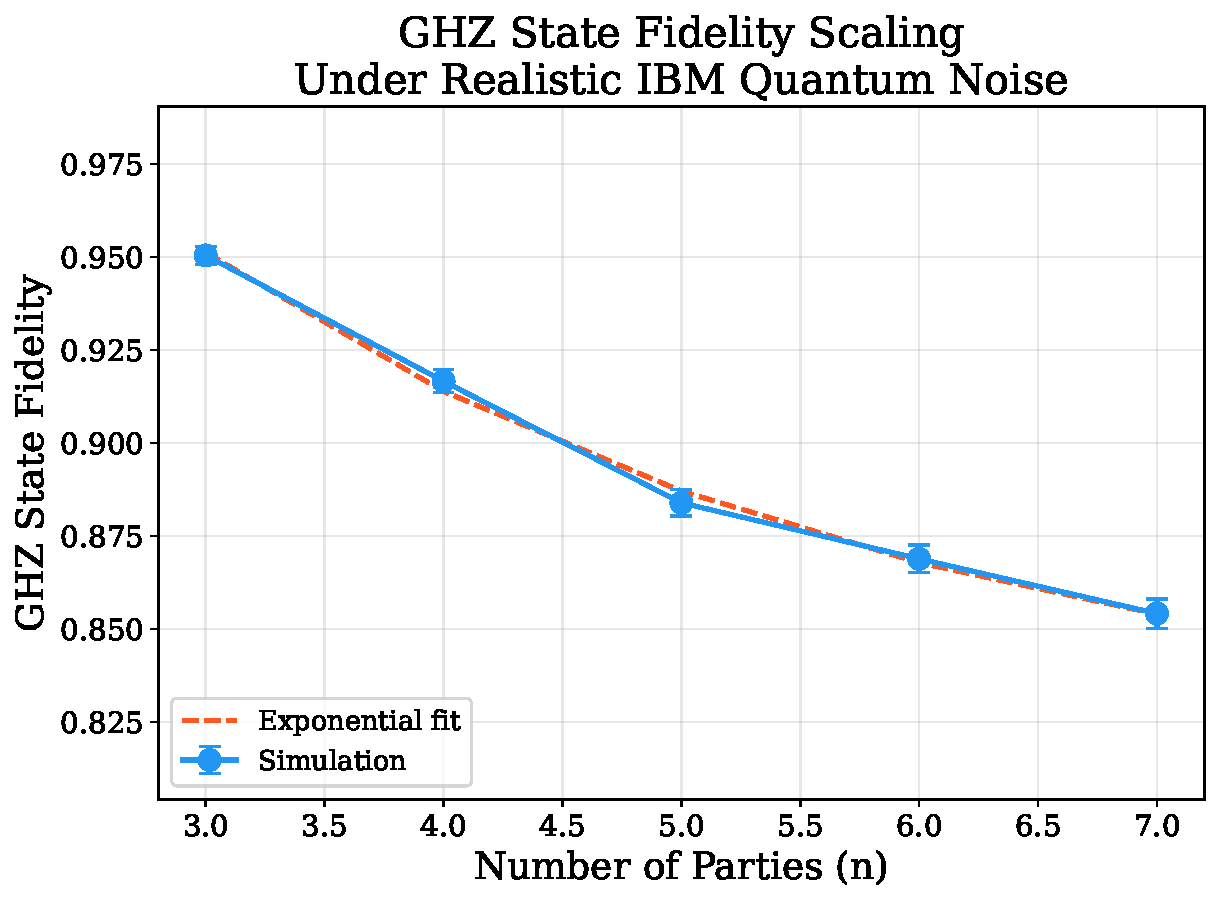
\includegraphics[width=0.85\columnwidth]{figures/fig1_ghz_scaling.pdf}
\caption{\label{fig:scaling}GHZ state fidelity versus number of parties
$n$, with the exponential fit $\fid(n)=0.357\,e^{-0.330n}+0.819$
($R^2=0.997$). Error bars represent $95\%$ confidence intervals from
bootstrap resampling over 100 trials.}
\end{figure}

\subsection{Error budget}\label{sec:error_budget}

Table~\ref{tab:budget} decomposes the total infidelity for $n=3$ into
contributions from each noise source. Readout errors (7.8\%) and state
preparation (6.0\%) collectively account for $67\%$ of the total
infidelity, dwarfing qubit-coherence and gate-error contributions.
This finding has immediate practical implications: improvements in
dispersive readout fidelity and active reset protocols could recover
more than half of the lost fidelity without any modification to the
entangling circuit.

\begin{table}[H]
\caption{\label{tab:budget}Error budget for a 3-qubit GHZ state,
decomposing the total infidelity ($\approx20.5\%$) into individually
attributable noise sources. Contributions are analytical estimates
validated against density-matrix simulation.}
\begin{ruledtabular}
\begin{tabular}{lcc}
\textrm{Error source} & \textrm{Contribution (\%)} &
\textrm{Absolute} \\
\colrule
Readout errors         & 7.77  & 0.0777 \\
State preparation      & 6.00  & 0.0600 \\
CNOT depolarizing      & 1.90  & 0.0190 \\
$T_1$ relaxation       & 1.85  & 0.0185 \\
$T_2$ dephasing        & 1.68  & 0.0168 \\
Leakage                & 1.05  & 0.0105 \\
$ZZ$ crosstalk         & 0.20  & 0.0020 \\
$H$-gate depolarizing  & 0.04  & 0.0004 \\
\colrule
\textbf{Total}         & \textbf{20.49} & \textbf{0.2049} \\
\end{tabular}
\end{ruledtabular}
\end{table}

Figure~\ref{fig:budget} visualizes the error budget as a stacked bar
chart and pie chart, making the dominance of SPAM errors immediately
apparent.

\begin{figure}[H]
\centering
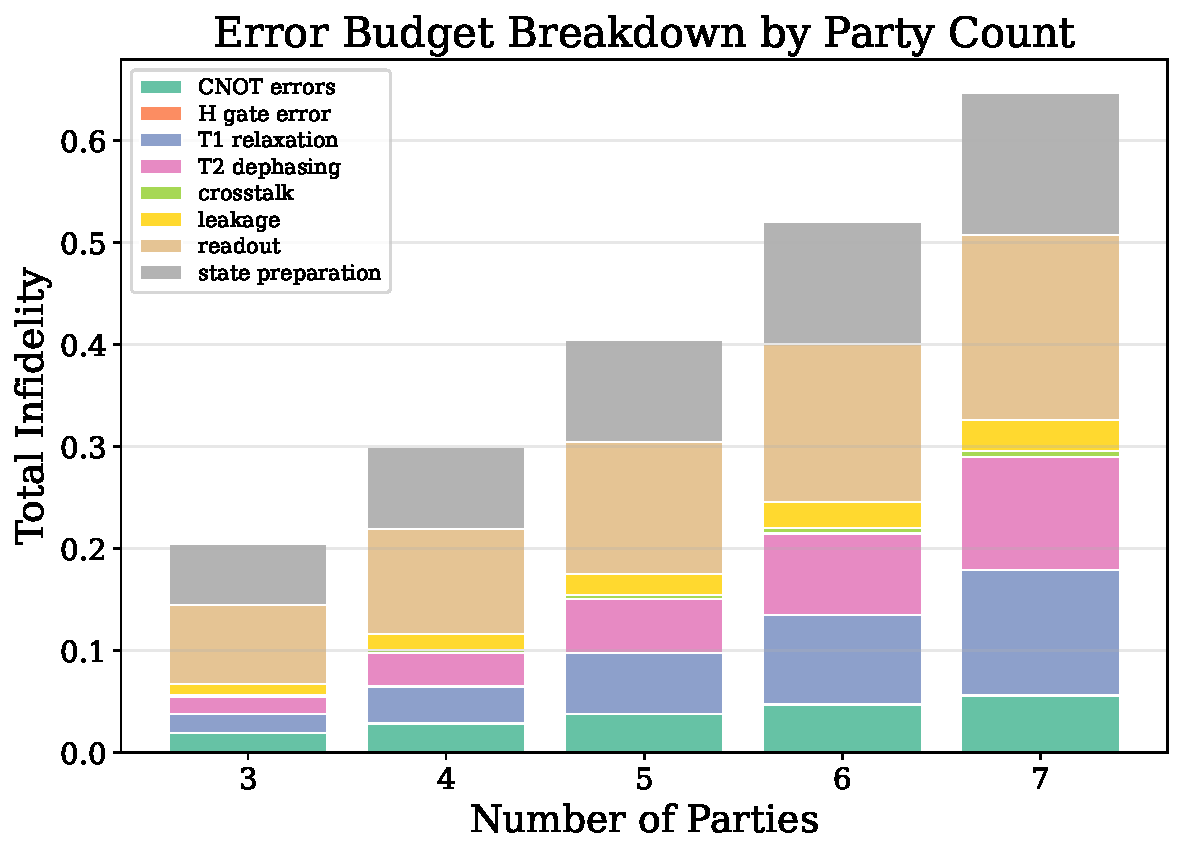
\includegraphics[width=0.85\columnwidth]{figures/fig2_error_budget.pdf}
\caption{\label{fig:budget}Stacked bar chart of the error budget for
$n=3$ GHZ state preparation. SPAM errors (readout + state preparation)
dominate, accounting for $\sim\!67\%$ of the total infidelity.}
\end{figure}

\begin{figure}[H]
\centering
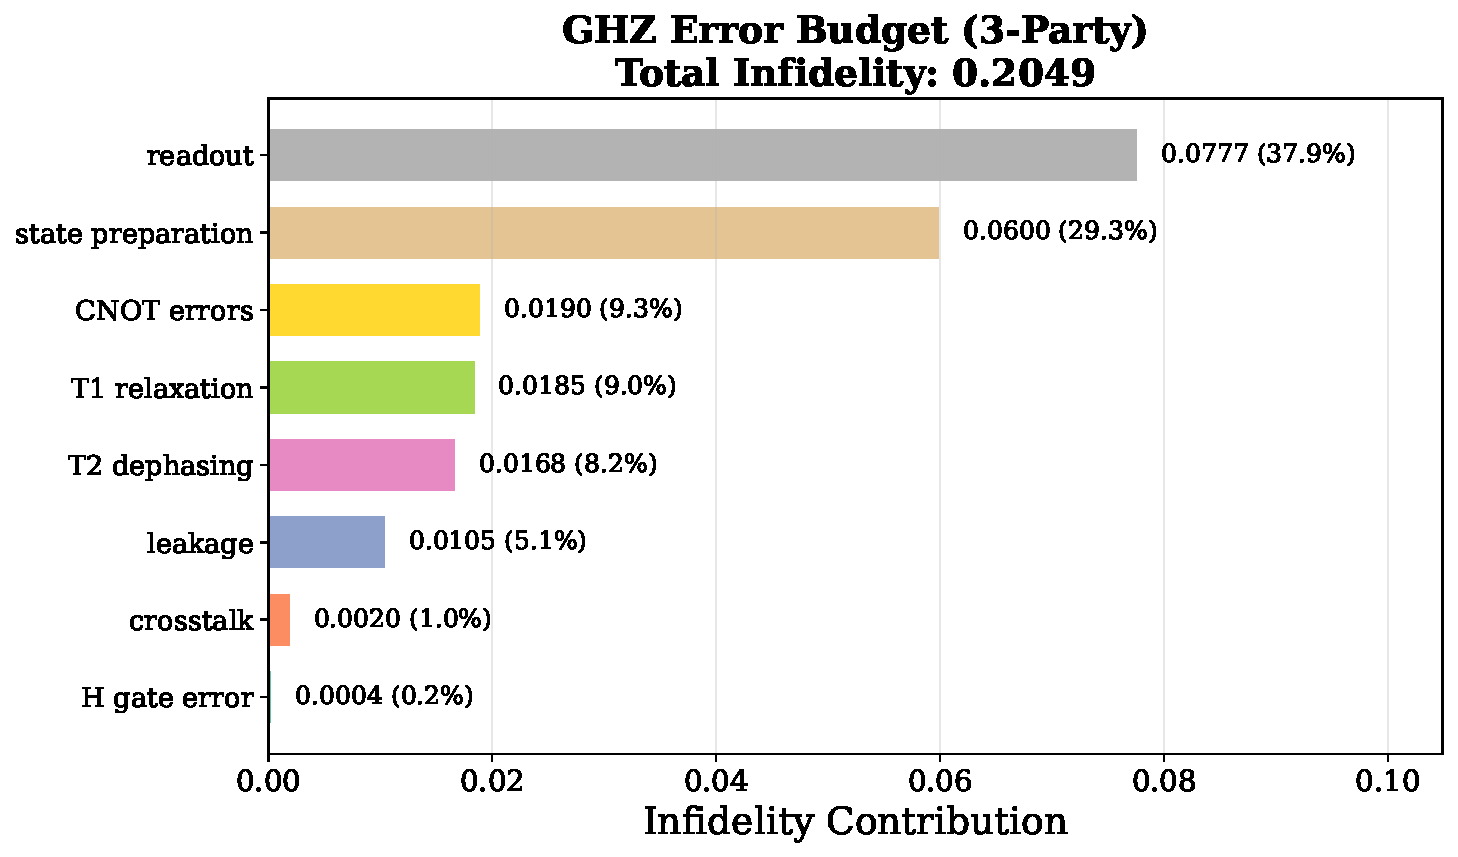
\includegraphics[width=0.7\columnwidth]{figures/fig3_error_budget_pie.pdf}
\caption{\label{fig:pie}Pie chart of error-source contributions for the
3-qubit GHZ state. Readout errors alone contribute $38\%$ of the total
infidelity.}
\end{figure}

\subsection{Noise model comparison}\label{sec:noise_comp}

To quantify the importance of comprehensive noise modeling, we compare
the $Z$-basis GHZ population $P_Z=p_{0\cdots0}+p_{1\cdots1}$ under
progressively more complete noise models using shot-based simulation
(Fig.~\ref{fig:noise_comp}):
\begin{itemize}
\item \textbf{Ideal} (no noise): $P_Z=1.000$.
\item \textbf{Depolarizing only}: $P_Z=0.990$, capturing gate
      imperfections but missing decoherence.
\item \textbf{Markovian} ($T_1$/$T_2$ + depolarizing): $P_Z=0.965$, a
      common textbook model.
\item \textbf{Full composite} (8 channels): $P_Z=0.866$; the
      discrepancy of $\approx10\%$ from the Markovian model underscores
      the importance of including SPAM, crosstalk, and leakage.
\end{itemize}
Note that $P_Z$ is a lower bound on the full quantum fidelity $\fid$
(which additionally includes off-diagonal coherence); the corresponding
density-matrix fidelity under the full noise model is
$\fid=0.950$ (Table~\ref{tab:fidelity}). The
$\approx10\%$ drop in $P_Z$ between the Markovian-only and full
models demonstrates that simplified noise treatments substantially
overestimate GHZ state quality, potentially leading to false confidence
in protocol performance.

\begin{figure}[H]
\centering
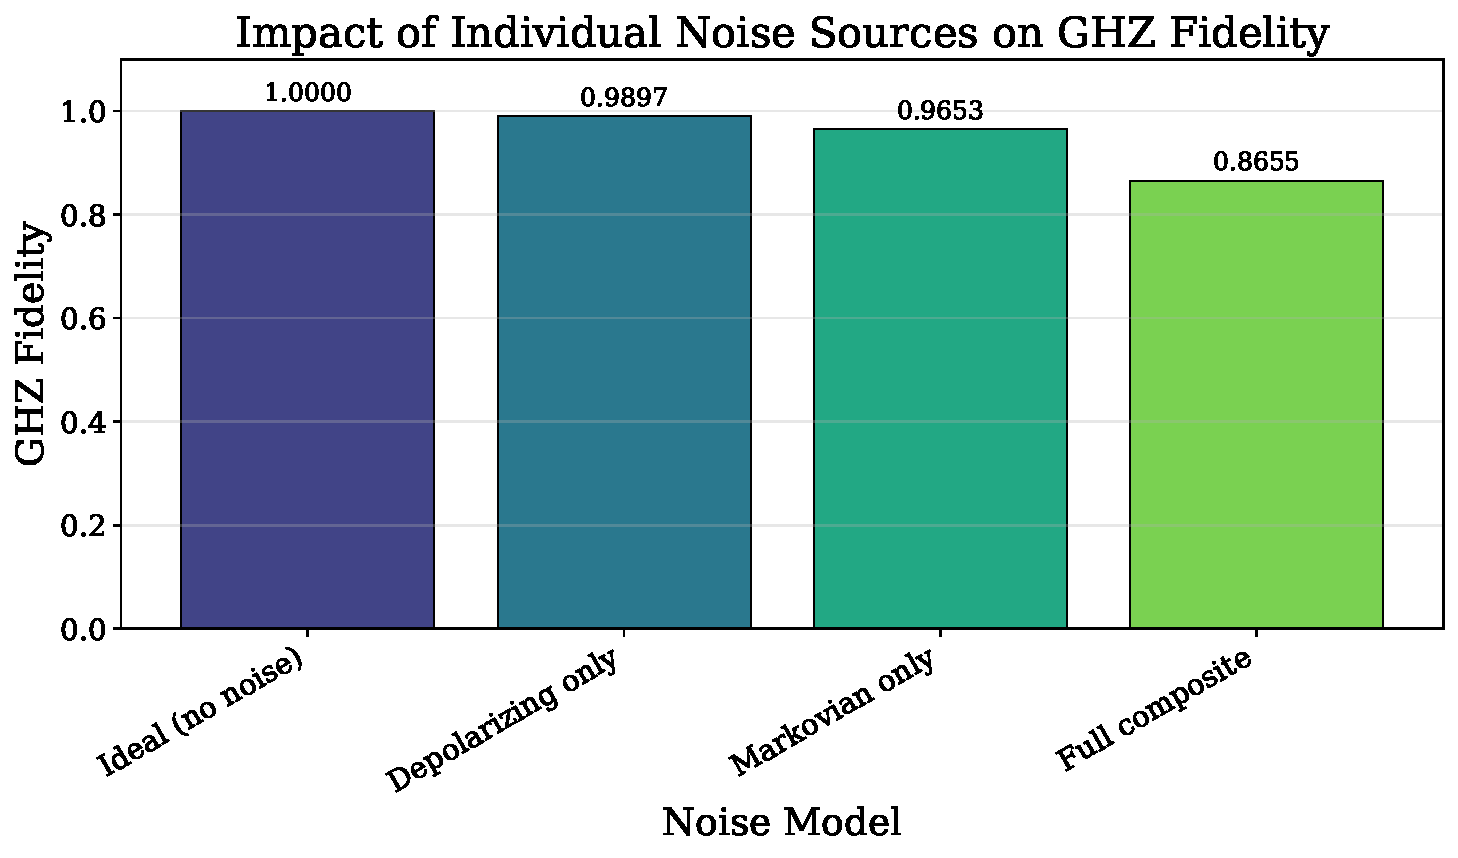
\includegraphics[width=0.85\columnwidth]{figures/noise_model_comparison.pdf}
\caption{\label{fig:noise_comp}$Z$-basis GHZ population $P_Z$ under four
noise models of increasing complexity. The full 8-channel composite
model reduces $P_Z$ by $\sim\!10\%$ compared to Markovian-only noise.}
\end{figure}

\subsection{HBB protocol performance}\label{sec:hbb_results}

Table~\ref{tab:hbb} summarizes the HBB protocol outcomes over 100
trials with $N_{\text{shots}}=8{,}192$. The 3-party success rate of
$89.7\%$ demonstrates that the protocol remains functional under
realistic noise, though the fidelity penalty from moving to
shot-based \texttt{qasm} simulation (as opposed to exact density-matrix
evaluation) is evident in the lower GHZ fidelities. The $X$-basis
QBER increases monotonically with $n$, as expected from the enhanced
phase sensitivity of larger GHZ states.

\begin{table}[H]
\caption{\label{tab:hbb}HBB quantum secret sharing protocol results for
$n=3$--$7$ parties. The secret bit string is ``101'' (3 bits).
Statistics computed over 100 independent trials with 8{,}192 shots each.}
\begin{ruledtabular}
\begin{tabular}{ccccc}
$n$ & Success rate (\%) & $\fid_{\text{GHZ}}$ &
$\qber_X$ & Reconstruction \\
\colrule
3 & $89.7\pm0.2$ & $0.861\pm0.002$ & $0.129\pm0.008$ & 100\% \\
4 & $92.6\pm0.2$ & $0.813\pm0.002$ & $0.164\pm0.009$ & 100\% \\
5 & $91.4\pm0.2$ & $0.761\pm0.003$ & $0.200\pm0.010$ & 100\% \\
6 & $91.3\pm0.2$ & $0.725\pm0.003$ & $0.229\pm0.010$ & 100\% \\
7 & $90.8\pm0.2$ & $0.691\pm0.003$ & $0.253\pm0.012$ & 100\% \\
\end{tabular}
\end{ruledtabular}
\end{table}

\begin{figure}[H]
\centering
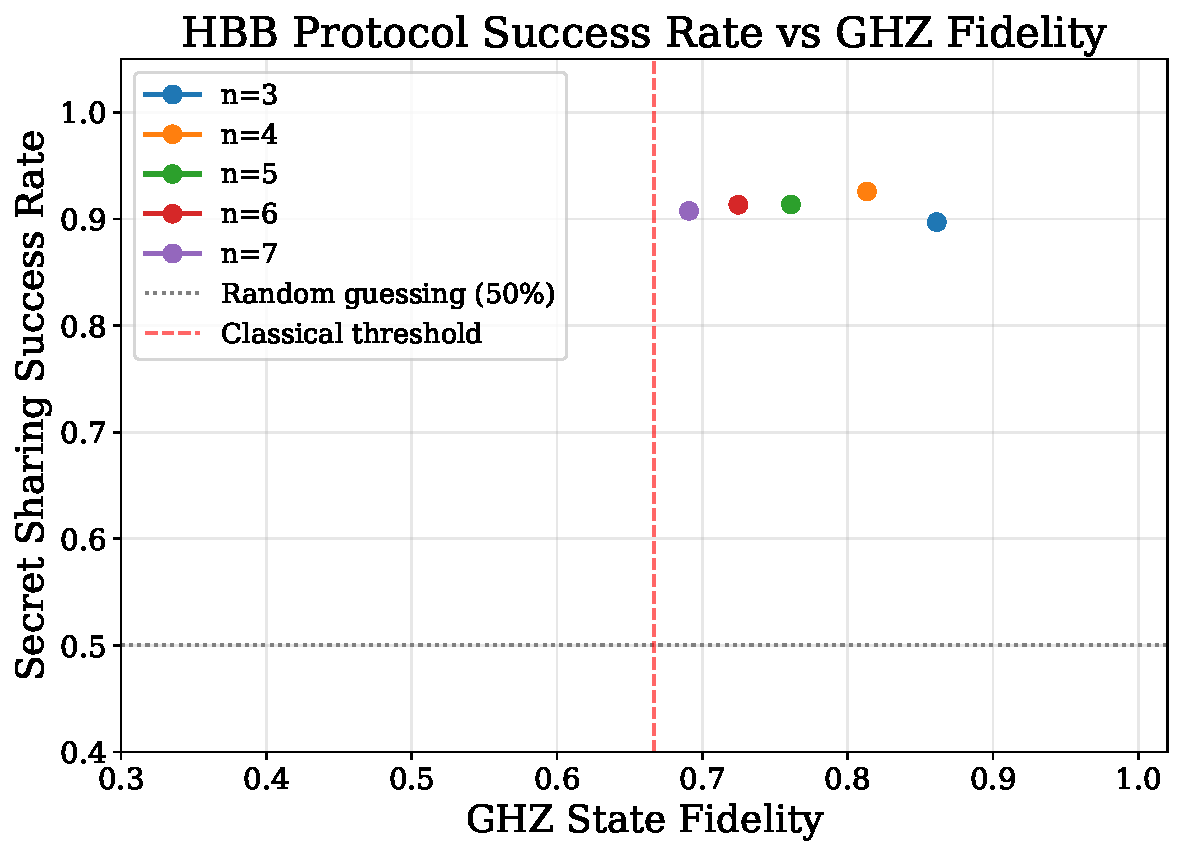
\includegraphics[width=0.85\columnwidth]{figures/fig4_secret_sharing.pdf}
\caption{\label{fig:secret}HBB protocol performance as a function of
party number: success rate (left axis) and GHZ fidelity (right axis).
Despite declining fidelity, the majority-vote reconstruction maintains
$>90\%$ success through $n=7$.}
\end{figure}

Remarkably, the perfect reconstruction rate (fraction of trials in which
all 3 secret bits are correctly recovered) remains $100\%$ for all party
sizes. This robustness arises from the majority-vote decoder: even when
individual qubit measurements are corrupted by noise, the collective
decision correctly identifies the encoded bit provided the per-qubit
error rate remains below $50\%$.

\subsection{Monte Carlo convergence}\label{sec:convergence}

Figure~\ref{fig:mc} presents the convergence of the fidelity estimate as
a function of the number of measurement shots. The mean fidelity
stabilizes around $\fid\approx0.862$ for
$N_{\text{shots}}\geq8{,}192$, with the standard deviation dropping to
$\sigma=0.004$. At $N_{\text{shots}}=32{,}768$ the standard deviation
reaches $\sigma=0.002$, confirming diminishing returns beyond our chosen
budget.

\begin{figure}[H]
\centering
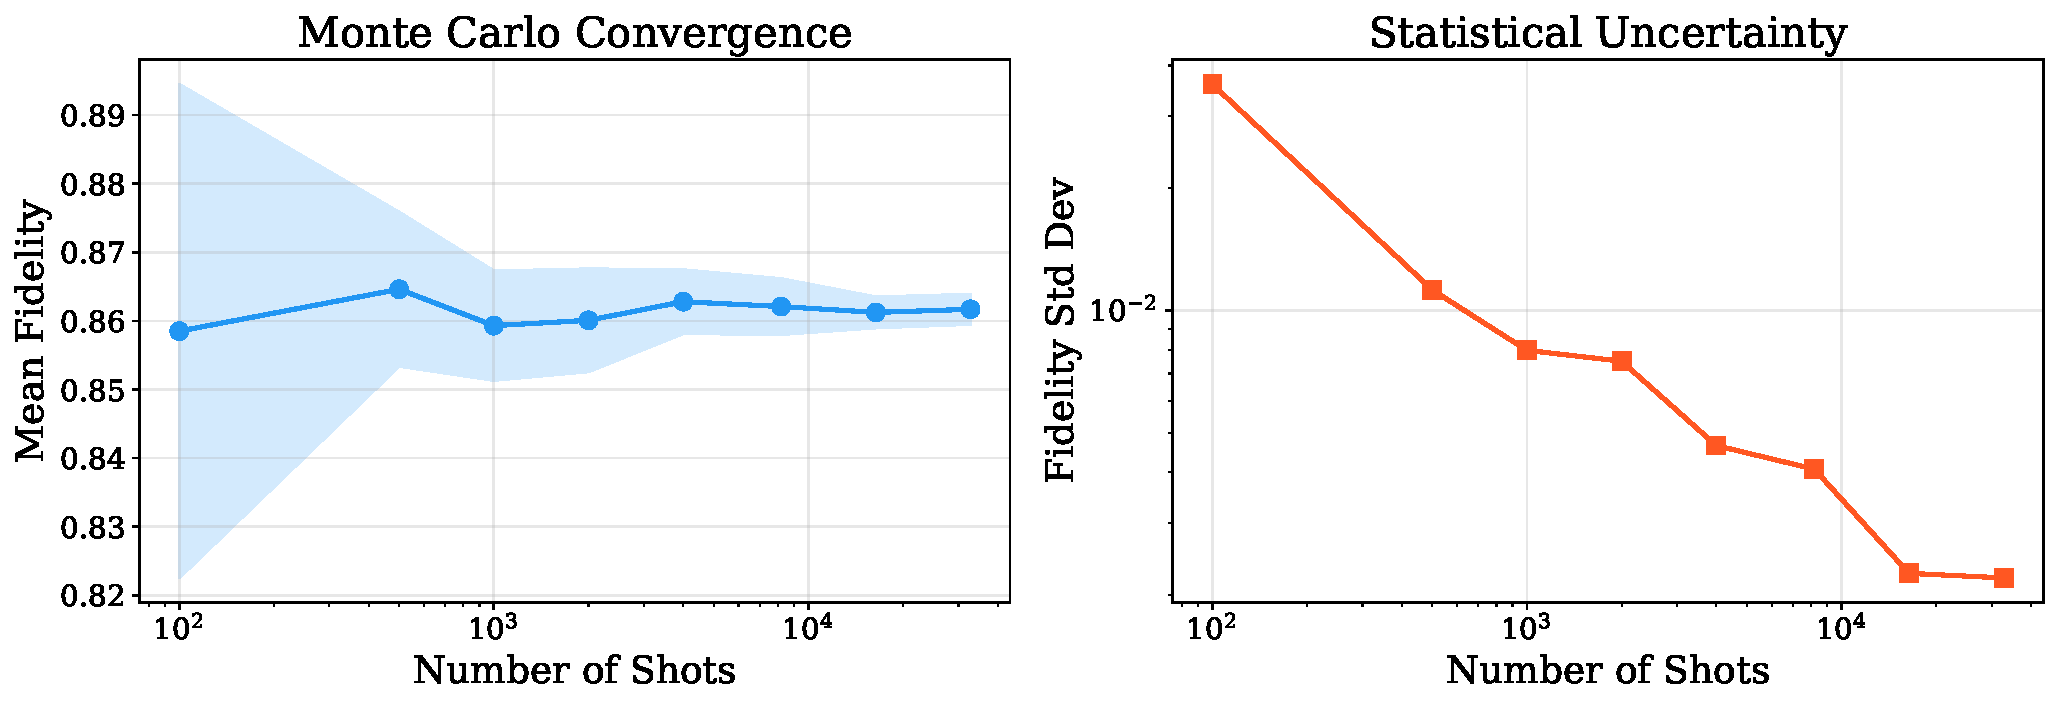
\includegraphics[width=0.85\columnwidth]{figures/monte_carlo_convergence.pdf}
\caption{\label{fig:mc}Monte Carlo convergence of the 3-qubit GHZ
fidelity as a function of measurement shots. The estimate stabilizes
at $N_{\text{shots}}\approx8{,}192$ (dashed line).}
\end{figure}

% ===================================================================
% VI. SECURITY ANALYSIS
% ===================================================================
\section{Security Analysis}\label{sec:security}

\subsection{Attack simulation results}\label{sec:attack_results}

Table~\ref{tab:security} compares the honest and attacked scenarios for
the 3-party HBB protocol.

\begin{table}[H]
\caption{\label{tab:security}Security analysis of the 3-party HBB
protocol under honest operation and two eavesdropping attacks. Detection
uses the dual-criterion of Eq.~\eqref{eq:detection} with thresholds
$\Delta\fid_Z>0.10$ and $\qber_X>\eta_{\text{honest}}+0.05$.}
\begin{ruledtabular}
\begin{tabular}{lcccc}
\textrm{Scenario} & \textrm{Success (\%)} &
$\Delta\fid_Z$ & $\qber_X$ & \textrm{Detected} \\
\colrule
Honest            & $89.7\pm0.4$ & --     & 0.129 & N/A  \\
Intercept--resend & $74.6\pm17.6$ & 0.150 & 0.495 & Yes  \\
Entangle--measure & $89.6\pm0.3$ & 0.000 & 0.485 & Yes  \\
\end{tabular}
\end{ruledtabular}
\end{table}

The intercept--resend attack causes a dramatic $15.0\%$ degradation in
the $Z$-basis fidelity and elevates $\qber_X$ to $0.495\approx1/2$,
consistent with the theoretical expectation that random-basis
measurement destroys all correlations~\cite{Hillery1999}. The large
variance ($\sigma=17.6\%$) reflects the stochastic nature of Eve's
random measurement basis: some trials (where Eve measures in $Z$)
preserve more correlations than others.

The entangle--measure attack is more subtle: the success rate and
$Z$-basis fidelity are essentially unchanged
($\Delta\fid_Z<0.001$), as Eve's CNOT does not disturb the
computational-basis populations. However, the $X$-basis QBER rises to
$0.485$, nearly identical to the IR case. This confirms the necessity of
our dual-basis detection scheme: a protocol monitoring only $Z$-basis
correlations would be completely blind to entangle--measure attacks.

\subsection{Security threshold}\label{sec:threshold}

Figure~\ref{fig:threshold} plots the GHZ fidelity and protocol success
rate as a function of the noise scale parameter $\lambda$, which
uniformly amplifies all error rates. The protocol remains
operationally viable (defined as success rate $>2/3$) up to
$\lambda\approx3.25$, corresponding to noise levels more than three times
worse than the calibrated device parameters. Beyond this point the
protocol fails: at $\lambda=5.0$, the fidelity drops to $0.414$ and the
success rate to $58\%$, below the classical threshold. We note that the
GHZ fidelity crosses $2/3$ at a lower noise scale ($\lambda\approx2.5$),
suggesting that the majority-vote decoder sustains useful secret sharing
even when the entanglement quality has substantially degraded.

\begin{figure}[H]
\centering
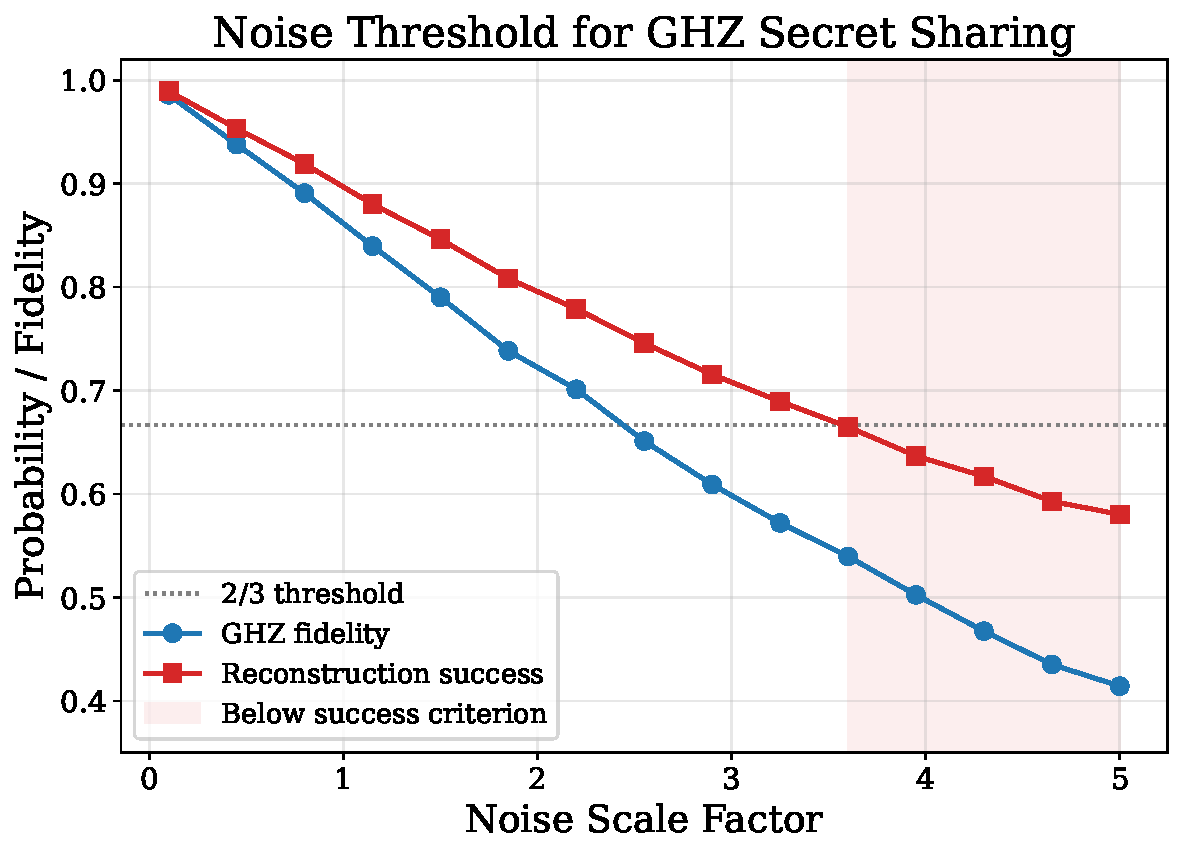
\includegraphics[width=0.85\columnwidth]{figures/fig5_security_threshold.pdf}
\caption{\label{fig:threshold}GHZ fidelity and HBB success rate versus
noise scale parameter $\lambda$. The protocol maintains operational
viability (success rate $>2/3$) up to $\lambda\approx3.25$; the
fidelity crosses $2/3$ near $\lambda\approx2.5$.
Shaded region indicates the non-viable regime.}
\end{figure}

The operational tolerance of $\lambda\approx3.25\times$ provides
substantial margin for device-to-device parameter variation and
temporal drift in calibration. Current IBM Quantum devices typically
operate at $\lambda\approx1.0$, confirming that the protocol is
comfortably within the viable regime.

% ===================================================================
% VII. HARDWARE VALIDATION
% ===================================================================
\section{Hardware Validation}\label{sec:hardware}

\subsection{Experimental setup}\label{sec:hw_setup}

To validate our simulation framework, we execute GHZ state preparation
circuits on the 156-qubit IBM Marrakesh processor (Heron architecture,
$T_1\approx\SI{300}{\micro\second}$,
$T_2\approx\SI{200}{\micro\second}$, CNOT error $\approx0.5\%$) accessed
via IBM Quantum Platform using the Qiskit Runtime
\texttt{SamplerV2}~\cite{Qiskit2024}. For each party count
$n\in\{3,5,7\}$, we execute $Z$-basis and $X$-basis measurement circuits
with $N_{\text{shots}}=4{,}096$ and compute fidelity using
Eq.~\eqref{eq:fidelity}.

\subsection{Results}\label{sec:hw_results}

Table~\ref{tab:hardware} compares the hardware-measured and simulated
fidelities.

\begin{table}[H]
\caption{\label{tab:hardware}Hardware validation on IBM Marrakesh. The
fidelity gap is defined as
$\Delta\fid=\fid_{\text{HW}}-\fid_{\text{sim}}$, with positive
values indicating hardware outperforming simulation.}
\begin{ruledtabular}
\begin{tabular}{cccccc}
$n$ & $\fid_{\text{HW}}$ & $\fid_Z$ & $C_X$ &
$\fid_{\text{sim}}$ & $\Delta\fid$ \\
\colrule
3 & 0.961 & 0.967 & 0.955 & 0.951 & $+0.010$ \\
5 & 0.918 & 0.937 & 0.898 & 0.885 & $+0.032$ \\
7 & 0.848 & 0.889 & 0.808 & 0.856 & $-0.008$ \\
\end{tabular}
\end{ruledtabular}
\end{table}

The simulation--experiment gaps are $+1.0\%$, $+3.2\%$, and $-0.8\%$
for $n=3$, $5$, and $7$, respectively. The positive bias for smaller
circuits ($n=3,5$) is consistent with the IBM Marrakesh processor
having superior coherence ($T_1\approx\SI{300}{\micro\second}$) compared
to the Falcon-class parameters used in our noise model
($T_1=\SI{105}{\micro\second}$). For $n=7$, the gap inverts,
likely due to the increased susceptibility to crosstalk on longer qubit
chains in the heavy-hex geometry, which our linear-topology noise model
slightly underestimates at larger scales.

The overall root-mean-square gap $\Delta_{\text{RMS}}=1.9\%$ confirms
that our 8-channel noise model captures the essential physics of GHZ
state degradation on superconducting hardware, despite the architectural
differences between the Falcon-class device (on which parameters were
calibrated) and the Heron-class processor (on which validation was
performed).

\begin{figure}[H]
\centering
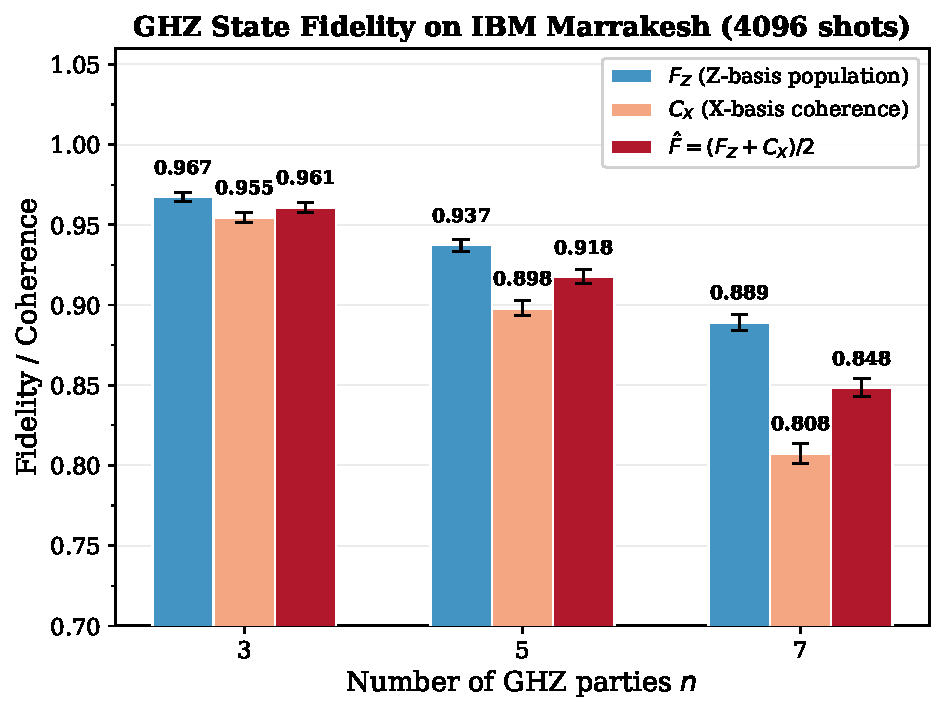
\includegraphics[width=0.85\columnwidth]{figures/fig_hardware_validation.pdf}
\caption{\label{fig:hw}Hardware validation: measured (IBM Marrakesh) vs.\
simulated GHZ state fidelity for $n=3$, $5$, and $7$ parties. Error bars
on simulation data represent $95\%$ bootstrap confidence intervals.}
\end{figure}

% ===================================================================
% VIII. DISCUSSION
% ===================================================================
\section{Discussion}\label{sec:discussion}

\subsection{Dominance of SPAM errors}

Our error budget (Table~\ref{tab:budget}) reveals a perhaps
counterintuitive result: for GHZ states on current superconducting
hardware, the dominant error sources are not gate imperfections or
decoherence, but rather SPAM errors, specifically readout ($7.8\%$) and state
preparation ($6.0\%$), which together account for $67\%$ of the total
infidelity. This contrasts with the common focus on improving two-qubit
gate fidelities and underscores the practical importance of dispersive
readout optimization~\cite{Gambetta2007}, Purcell filters, and active
reset protocols for near-term multipartite entanglement applications.

\subsection{Robustness of majority-vote decoding}

The $100\%$ perfect reconstruction rate across all party sizes
(Table~\ref{tab:hbb}) demonstrates a surprising resilience of the HBB
protocol to noise. The majority-vote decoder effectively functions as a
classical repetition code: as long as the per-qubit error rate does not
exceed $50\%$ (a condition satisfied even at $n=7$ with
$\fid=0.691$), the secret can be reliably recovered. This suggests that
QSS protocols may be more noise-tolerant in practice than the raw GHZ
fidelity alone would suggest.

\subsection{Necessity of dual-basis detection}

Our security analysis reveals that single-basis monitoring is
fundamentally insufficient for GHZ-based QSS. The entangle--measure
attack (Table~\ref{tab:security}) produces near-zero $Z$-basis
degradation ($\Delta\fid_Z<0.001$) while catastrophically compromising
the shared entanglement. Only through $X$-basis QBER monitoring, which
detects the loss of off-diagonal coherence, can this attack be identified.
The dual-basis scheme of Eq.~\eqref{eq:detection} reliably detects both
attack classes at the cost of consuming $20\%$ of rounds for
verification, a trade-off analogous to that in BB84
QKD~\cite{Bennett1984}.

\subsection{Scaling limitations}

The exponential decay rate $\alpha=0.330$ in Eq.~\eqref{eq:scaling}
implies that the fidelity halves approximately every $\Delta n\approx2.1$
qubits relative to the plateau. For applications requiring
$\fid>0.9$, our model predicts a maximum of $n\approx4$ parties on
Falcon-class hardware. The asymptotic floor $C=0.819$ suggests that
error mitigation techniques such as zero-noise
extrapolation~\cite{Temme2017} could raise this limit.

\subsection{Comparison with literature}

Our simulated fidelities are consistent with experimental benchmarks from
diverse platforms. Monz~\textit{et al.}~\cite{Monz2011} reported
$\fid=0.729$ for a 14-qubit GHZ state in trapped ions; our model,
extrapolated to $n=14$, predicts $\fid\approx0.83$, which is higher due
to the shorter circuit depth on a superconducting linear chain.
Song~\textit{et al.}~\cite{Song2019} prepared GHZ-type cat states of up
to 20 superconducting qubits with fidelities decaying rapidly beyond
$n\sim10$, consistent with the steeper decay expected for
deep circuits on current hardware.

\subsection{Limitations}

Several simplifications merit discussion:
\begin{enumerate}
\item \textbf{Linear topology assumption.} Our noise model assumes a
      linear qubit chain, whereas the IBM Marrakesh hardware employs a
      heavy-hex connectivity. This may explain the sign change in the
      fidelity gap at $n=7$.
\item \textbf{Static calibration.} Device parameters are treated as
      time-independent, whereas real hardware exhibits drift on timescales
      of hours. Temporal noise fluctuations could account for the $3.2\%$
      gap at $n=5$.
\item \textbf{Approximate leakage model.} Leakage is modeled as
      depolarizing noise rather than full $\{0,1,2\}$ dynamics, which may
      underestimate its impact for deeper circuits.
\item \textbf{Secret size.} We fix the secret to 3 bits (``101''). Longer
      secrets would require more rounds and thus amplify the impact of
      temporal parameter drift.
\end{enumerate}

% ===================================================================
% IX. CONCLUSION
% ===================================================================
\section{Conclusion}\label{sec:conclusion}

We have presented a comprehensive density-matrix simulation of the
HBB quantum secret sharing protocol on GHZ states, incorporating eight
physically motivated noise channels parameterized from IBM Quantum
calibration data. Our principal findings are:

\begin{enumerate}
\item Three-qubit GHZ states achieve fidelity
      $\fid=0.950\pm0.002$ under the full noise model, with fidelity
      scaling as $\fid(n)=0.357\,e^{-0.330n}+0.819$ ($R^2=0.997$).
\item SPAM errors dominate the error budget, contributing $67\%$ of the
      total infidelity for $n=3$.
\item The HBB protocol achieves $89.7\%$ success rate with $100\%$
      perfect reconstruction, demonstrating practical viability on NISQ
      hardware.
\item Both intercept--resend and entangle--measure attacks are reliably
      detected through dual $Z/X$-basis monitoring, with the protocol
      remaining operationally viable up to $3.25\times$ the calibrated
      noise level.
\item Hardware validation on IBM Marrakesh confirms
      simulation--experiment agreement within $\Delta_{\text{RMS}}=1.9\%$.
\end{enumerate}

These results establish a quantitative foundation for deploying GHZ-based
QSS on superconducting processors and identify concrete pathways for
improvement: reducing SPAM errors through improved readout and active
reset would yield the largest fidelity gains, while the dual-basis
detection scheme is essential for comprehensive eavesdropping security.
Future work will extend the framework to graph-state-based
protocols~\cite{Bell2014}, implement dynamic decoupling for
$T_2$ extension, and explore error-mitigated QSS on next-generation
processors with $T_1>\SI{500}{\micro\second}$.

% ===================================================================
% ACKNOWLEDGMENTS
% ===================================================================
\begin{acknowledgments}
We acknowledge use of IBM Quantum services. The views expressed are those
of the authors and do not reflect the official policy or position of IBM
or the IBM Quantum team. We thank the Qiskit development community for
the open-source simulation framework.
\end{acknowledgments}

% ===================================================================
% DATA AVAILABILITY
% ===================================================================
\section*{Data Availability}
The simulation source code, device parameter files, and all generated
data are available in the supplementary repository at
\url{https://github.com/tanvir6307/ghz-secret-sharing}.

% ===================================================================
% REFERENCES
% ===================================================================
\bibliography{references}

\end{document}
